\documentclass[12pt]{article}
\usepackage[a4paper]{geometry}
\usepackage{fullpage}
\usepackage[T1]{fontenc}
\usepackage[utf8]{inputenc}
\usepackage{graphicx}
\usepackage{mathpazo}
\pagenumbering{gobble}
\usepackage{siunitx}
\DeclareSIUnit\voltampere{VA}
\usepackage{amsmath}
\usepackage[spanish]{babel}
\usepackage{steinmetz}
\usepackage{enumitem}
\usepackage{diffcoeff}

\begin{document}

\title{}

\section{Transitorio de primer orden}

\subsection{FM 4.2}

Calcular la corriente $i(t)$ para $t > 0$. 

\begin{minipage}{0.5\textwidth}
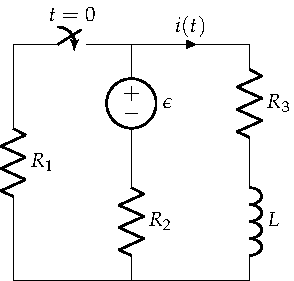
\includegraphics{figs/FM_4_2}
\end{minipage}
\hfill
\begin{minipage}{0.5\textwidth}
Datos:
\begin{align*}
  \epsilon &= \SI{24}{\volt}\\
  R_1 &= \SI{8}{\ohm}\\
  R_2 &= \SI{4}{\ohm}\\
  R_3 &= \SI{4}{\ohm}\\
  L &= \SI{15}{\henry}
\end{align*}
\end{minipage}

\subsubsection*{Solución}

Calculamos las condiciones iniciales ($t = 0^-$)

Dibujamos el circuito para $t < 0$ y obtenemos:

\begin{minipage}{0.3\textwidth}
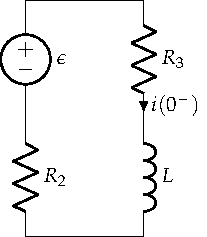
\includegraphics{figs/FM_4_2_t0-}
\end{minipage}
\begin{minipage}{0.7\textwidth}
  \begin{equation*}
    i(t) = \frac{\epsilon}{R_2 + R_3}
  \end{equation*}
\end{minipage}

Por tanto, $i(0^-) = \SI{3}{\ampere}$. Al tratarse de una bobina, $i(0^+) = i(0^-) = \SI{3}{\ampere}$.

A continuación dibujamos el circuito para $t > 0$ para obtener la respuesta natural y la respuesta forzada.

Para obtener la respuesta natural apagamos las fuentes. En este circuito obtenemos:

\begin{minipage}{0.3\textwidth}
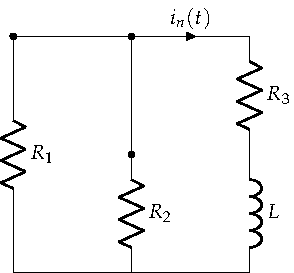
\includegraphics{figs/FM_4_2_natural}
\end{minipage}
\begin{minipage}{0.7\textwidth}
  \begin{align*}
    R_{th} &= R_3 + R_1||R_2 = 20/3\si{\ohm}\\
    \tau &= L/R_{th} = 9/4\si{\second}\\
    i_n(t) &= A \cdot e^{-\frac{t}{\tau}} = A \cdot e^{-4t/9}
  \end{align*}
\end{minipage}
Queda por determinar la constante de integración.

Para obtener la respuesta forzada volvemos a activar las fuentes. En este circuito obtenemos:

\begin{minipage}{0.3\textwidth}
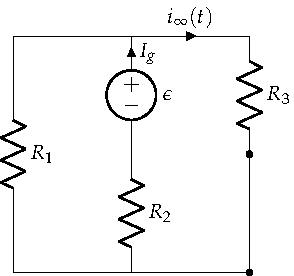
\includegraphics{figs/FM_4_2_forzada}
\end{minipage}
\begin{minipage}{0.7\textwidth}
  \begin{align*}
    I_g &= \frac{\epsilon}{R_2 + R_1||R_3}\\
    i_\infty(t) &= I_g \cdot \frac{G_3}{G_3 + G_1} = \SI{2.4}{\ampere}
  \end{align*}
\end{minipage}

Con estos dos resultados podemos obtener la respuesta completa:

\begin{align*}
  i(t) &= i_n(t) + i_\infty(t)\\
  i(t) &= A \cdot e^{-4t/9} + 2.4
\end{align*}

Para determinar la constante de integración recurrimos a las condiciones iniciales:

\begin{align*}
  i(0^+) &= A + 2.4\\
  i(0^+) &= 3\\
  A &= 0.6
\end{align*}

Por tanto,

\begin{equation*}
  i(t) = 0.6 \cdot e^{-4t/9} + 2.4
\end{equation*}

\clearpage

\subsection{FM 4.3}

Calcular la tensión en bornes del condensador para $t > 0$.

\begin{minipage}{0.5\textwidth}
  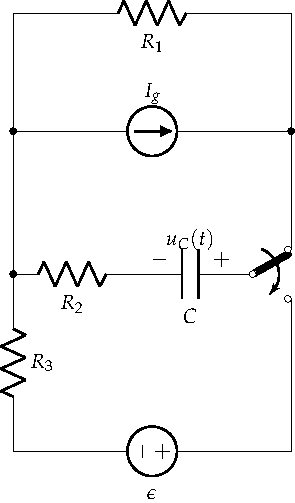
\includegraphics[scale=0.85]{figs/FM_4_3}
\end{minipage}
\hfill
\begin{minipage}{0.5\textwidth}
Datos:
\begin{align*}
  \epsilon &= \SI{20}{\volt}\\
  I_g &= \SI{4}{\ampere}\\
  R_1 &= \SI{6}{\ohm}\\
  R_2 &= \SI{4}{\ohm}\\
  R_3 &= \SI{12}{\ohm}\\
  C &= \SI[parse-numbers=false]{1/16}{\farad}      
\end{align*}

\end{minipage}

\subsubsection*{Solución}

Calculamos las condiciones iniciales ($t = 0^-$)

Dibujamos el circuito para $t < 0$ y obtenemos:

\begin{minipage}{0.3\textwidth}
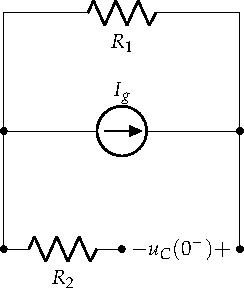
\includegraphics{figs/FM_4_3_t0-}
\end{minipage}
\begin{minipage}{0.7\textwidth}
  \begin{equation*}
    u_C(t) = I_g \cdot R_1 
  \end{equation*}
\end{minipage}

Por tanto, $u_c(0^-) = \SI{24}{\volt}$. Al tratarse de un condensador, $u_C(0^+) = u_C(0^-) = \SI{24}{\volt}$.

A continuación dibujamos el circuito para $t > 0$ para obtener la respuesta natural y la respuesta forzada.

Para obtener la respuesta natural apagamos las fuentes. En este circuito obtenemos:

\begin{minipage}{0.3\textwidth}
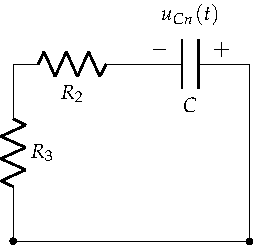
\includegraphics{figs/FM_4_3_natural}
\end{minipage}
\begin{minipage}{0.7\textwidth}
  \begin{align*}
    R_{th} &= R_2 + R_3 = \SI{16}{\ohm}\\
    \tau &= C/G_{th} = \SI{1}{\second}\\
    u_{Cn}(t) &= A \cdot e^{-\frac{t}{\tau}} = A \cdot e^{-t}
  \end{align*}
\end{minipage}
Queda por determinar la constante de integración.

Para obtener la respuesta forzada volvemos a activar las fuentes. En este circuito obtenemos:

\begin{minipage}{0.3\textwidth}
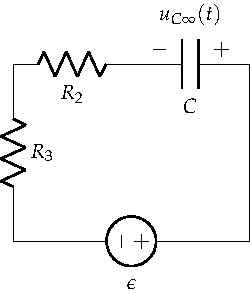
\includegraphics{figs/FM_4_3_forzada}
\end{minipage}
\begin{minipage}{0.7\textwidth}
  \begin{equation*}
    u_{c\infty}(t) = \epsilon = \SI{20}{\volt}
  \end{equation*}
\end{minipage}

Con estos dos resultados podemos obtener la respuesta completa:

\begin{align*}
  u_C(t) &= u_{Cn}(t) + u_{c\infty}(t)\\
  u_C(t) &= A \cdot e^{-t} + 20
\end{align*}

Para determinar la constante de integración recurrimos a las condiciones iniciales:

\begin{align*}
  u_C(0^+) &= A + 20\\
  u_C(0^+) &= 24\\
  A &= \SI{4}{\volt}
\end{align*}

Por tanto,

\begin{equation*}
  u_C(t) = 4 \cdot e^{-t} + 20
\end{equation*}

\clearpage

\subsection{HKD 8.4}

Determina las corrientes $i_L(t)$ e $i_1(t)$ para $t > 0$.

\begin{minipage}{0.7\textwidth}
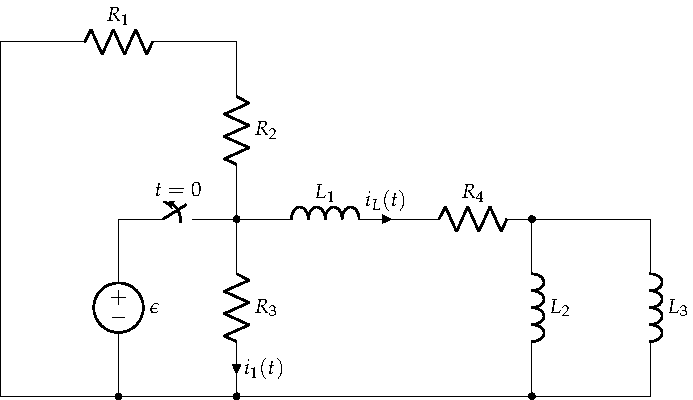
\includegraphics{figs/HKD84}
\end{minipage}
\hfill
\begin{minipage}{0.3\textwidth}
Datos:
\begin{align*}
  \epsilon &= \SI{18}{\volt}\\
  R_1 &= \SI{120}{\ohm}\\
  R_2 &= \SI{60}{\ohm}\\
  R_3 &= \SI{90}{\ohm}\\
  R_4 &= \SI{50}{\ohm}\\
  L_1 &= \SI{1}{\milli\henry}\\
  L_2 &= \SI{2}{\milli\henry}\\
  L_3 &= \SI{3}{\milli\henry}
\end{align*}
\end{minipage}

\subsubsection*{Solución}

Calculamos las condiciones iniciales ($t = 0^-$)

Dibujamos el circuito para $t < 0$:

\begin{center}
  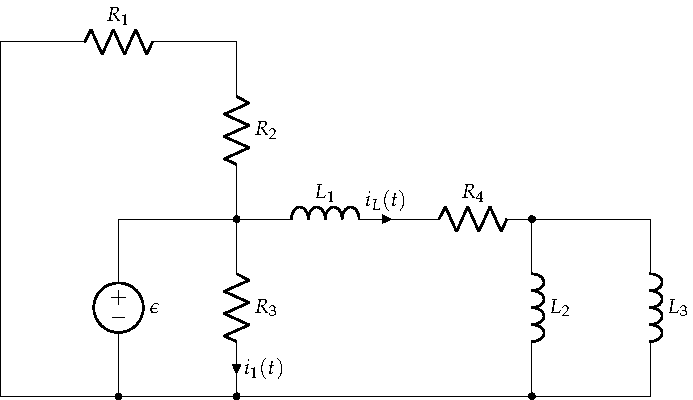
\includegraphics[scale=0.85]{figs/HKD84_t0-}
\end{center}

Obtenemos:
\begin{equation*}
  i_L(t) = \frac{\epsilon}{R_4} = \SI{360}{\milli\ampere}
\end{equation*}

Al tratarse de una bobina, $i_L(0^+) = i_L(0^-) = \SI{360}{\milli\ampere}$.

En este circuito podemos calcular $i_1(0^-) = \frac{\epsilon}{R_3} = \SI{200}{\milli\ampere}$. Este valor nos servirá de referencia cuando calculemos $i_1(t)$.

A continuación dibujamos el circuito para $t > 0$ para obtener la respuesta natural y la respuesta forzada. En el circuito resultante no hay fuentes, por lo que únicamente tendremos respuesta natural.

\begin{center}
  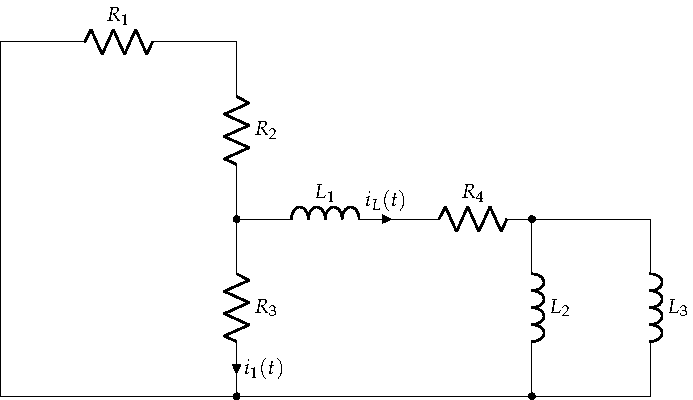
\includegraphics{figs/HKD84_natural}
\end{center}

  \begin{align*}
    L_{eq} &= L_1 + L_2||L_3 = \SI{2.2}{\milli\henry}\\
    R_{th} &= (R_1 + R_2) || R_3 + R_4  = \SI{110}{\ohm}\\
    \tau &= L_{eq}/R_{th} = \SI{20}{\micro\second}\\
    i_{Ln}(t) &= A \cdot e^{-\frac{t}{\tau}} = A \cdot e^{-5 \cdot 10^{-4} \cdot t}
  \end{align*}

Queda por determinar la constante de integración. Dado que la respuesta forzada es 0 podemos calcular directamente esta constante con la respuesta natural y las condiciones iniciales:


\begin{align*}
  i_L(t) &= i_{Ln}(t) = A \cdot e^{-5 \cdot 10^{-4} \cdot t}\\
  i_L(0^+) &= A = 0.36
\end{align*}

Por tanto,

\begin{equation*}
  i_L(t) = 0.36 \cdot e^{-5 \cdot 10^{-4} \cdot t}\si{\ampere}
\end{equation*}

Para calcular la corriente $i_1(t)$ usamos un divisor de corriente a partir de $i_L(t)$:

\begin{equation*}
  i_1(t) = -i_L(t) \cdot \frac{1/R_3}{1/R_3 + 1/(R_1 + R_2)} = -0.24 \cdot e^{-5 \cdot 10^{-4} \cdot t}\si{\ampere}
\end{equation*}

En el primer apartado habíamos obtenido $i_1(0^-) = \SI{200}{\milli\ampere}$. Con esta ecuación obtenemos $i_1(0^+) = -\SI{240}{\milli\ampere}$. Los valores no coinciden porque en una resistencia no hay condición de continuidad.

\clearpage

\section{Transitorio de segundo orden}

\subsection{FM 4.8}

El circuito de la figura ha alcanzado el régimen permanente con el interruptor cerrado. El interruptor se abre en $t = 0$. Calcula las expresiones de la tensión en bornes del condensador y de la corriente por la bobina para $t > 0$.

\vspace*{1cm}

\begin{minipage}{0.7\textwidth}
  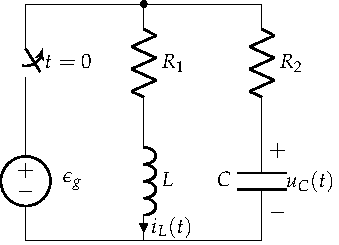
\includegraphics[scale=0.95]{figs/FM_4_8}
\end{minipage}
\hfill
\begin{minipage}{0.3\textwidth}
Datos:
\begin{align*}
  \epsilon_g &= \SI{10}{\volt}\\
  R_1 &= \SI{10}{\ohm}\\
  R_2 &= \SI{5}{\ohm}\\
  L &= \SI{2.5}{\henry}\\
  C &= \SI{0.2}{\farad}      
\end{align*}
\end{minipage}

\subsection*{Solución}

Calculamos las condiciones iniciales ($t = 0^-$)

Dibujamos el circuito para $t < 0$ y obtenemos:

\begin{minipage}{0.3\textwidth}
%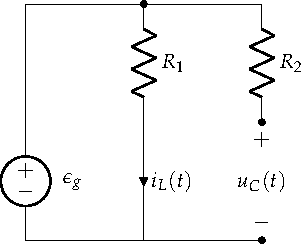
\includegraphics{figs/FM_4_8_t0-}
\end{minipage}
\begin{minipage}{0.7\textwidth}
  \begin{align*}
    u_C(t) &= \SI{10}{\volt}\\
    i_L(t) &= \frac{\epsilon_g}{R_1} = \SI{1}{\ampere}
  \end{align*}
\end{minipage}

Por tanto, $u_c(0^+) = u_c(0^-) = \SI{10}{\volt}$ y $i_L(0^+) = i_L(0^-) = \SI{1}{\ampere}$.

A continuación dibujamos el circuito para $t > 0$ para obtener la respuesta natural y la respuesta forzada. En el circuito resultante no hay fuentes, por lo que no habrá respuesta forzada.

\begin{minipage}{0.3\textwidth}
%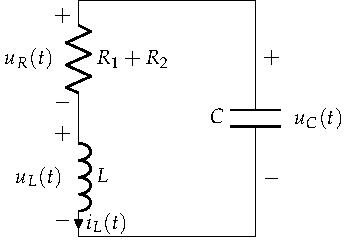
\includegraphics{figs/FM_4_8_natural}
\end{minipage}
\begin{minipage}{0.7\textwidth}
  \begin{align*}
    i_L(t) &= A_1 \cdot e^{s_1 \cdot t} + A_2 \cdot e^{s_2 \cdot t}\\
    s_1 &= -\alpha + \sqrt{\alpha^2 - \omega_0^2}\\
    s_2 &= -\alpha - \sqrt{\alpha^2 - \omega_0^2}\\
    \alpha &= \frac{R}{2L} = \SI{3}{\per\second}\\
    \omega_0 &= \frac{1}{\sqrt{LC}} = \sqrt{2}\si{\radian\per\second}
  \end{align*}
\end{minipage}

Dado que $\alpha > \omega_0$ se trata de un transitorio sobreamortiguado:

\begin{align*}
  s_1 &= \SI{-0.354}{\per\second}\\
  s_2 &= \SI{-5.645}{\per\second}\\
  i_L(t) &= A_1 \cdot e^{-0.354 \cdot t} + A_2 \cdot e^{-5.645 \cdot t}
\end{align*}

Para determinar las constantes de integración recurrimos a las condiciones iniciales:

\begin{align*}
  u_R(t) + u_L(t) &= u_C(t)\\
  u_L(0^+) &= u_C(0^+) - u_R(0^+)\\
  u_R(0^+) &= R \cdot i_L(0^+) = \SI{15}{\volt}\\
  u_L(0^+) &= 10 - 15 = \SI{-5}{\volt}
\end{align*}

Por tanto,

\begin{align*}
  i_L(0^+) &= \SI{1}{\ampere}\\
  \diff{i_L(t)}{t}{t = 0^+} &= \frac{1}{L} \cdot u_L(0^+) = \SI{-2}{\ampere\per\second}
\end{align*}

Con estos resultados, particularizamos la ecuación de $i_L(t)$ para $t = 0$ y así planteamos las ecuaciones para obtener $A_1$ y $A_2$:

\begin{align*}
  i_L(0^+) &= A_1 + A_2 = 1\\
  \diff{i_L(t)}{t}{t = 0^+} &= A_1 \cdot s_1 + A_2 \cdot s_2 = -2
\end{align*}

Por tanto,

\begin{align*}
  A_1 &= 0.689\\
  A_2 &= 0.311
\end{align*}

Finalmente,

\begin{equation*}
  i_L(t) = 0.689 \cdot e^{-0.354 \cdot t} + 0.311 \cdot e^{-5.645 \cdot t}\\
\end{equation*}

Para obtener la tensión en el condensador recurrimos a la LKV:

\begin{align*}
  u_C(t) &= u_R(t) + u_L(t) = \\
         &= R \cdot i_L(t) + L \diff{i_L(t)}{t} = \\
  &= 9.7275 \cdot e^{-0.354 \cdot t} + 0.275 \cdot e^{-5.645 \cdot t}
\end{align*}

\clearpage

\subsection{FM 4.9}

En el circuito de la figura, calcula la tensión $u_c(t)$ para $t > 0$.

\vspace*{1cm}

\begin{minipage}{0.7\textwidth}
  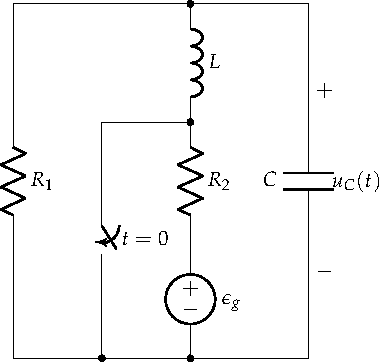
\includegraphics[scale=0.8]{figs/FM_4_9}
\end{minipage}
\hfill
\begin{minipage}{0.3\textwidth}
Datos:
\begin{align*}
  \epsilon_g &= \SI{4}{\volt}\\
  R_1 &= \SI{2}{\ohm}\\
  R_2 &= \SI{2}{\ohm}\\
  L &= \SI{2}{\henry}\\
  C &= \SI{0.25}{\farad}      
\end{align*}
\end{minipage}


\end{document}